\documentclass[11pt, a4paper]{article}

% Fonts and Encoding
\usepackage[utf8]{inputenc}
\usepackage[T1]{fontenc}

% Math and Symbols
\usepackage{amsmath, amssymb, amsthm, amsfonts, mathrsfs, mathtools}

% Layout and Geometry
\usepackage{geometry}
\geometry{a4paper, margin=1in}

% Formatting and Graphics
\usepackage{graphicx, xcolor, enumitem, booktabs, array, tabularx}

% TikZ for Illustrations
\usepackage{tikz}
\usetikzlibrary{arrows.meta, positioning, shapes.geometric, calc, backgrounds, matrix}

% Clickable Links and TOC
\usepackage{hyperref}
\hypersetup{
    colorlinks=true,
    linkcolor=blue,
    filecolor=magenta,      
    urlcolor=cyan,
    pdftitle={Theory of Higher-Order Linear Differential Equations},
}

% Theorem Environments
\newtheorem{theorem}{Theorem}[section]
\newtheorem{lemma}[theorem]{Lemma}
\newtheorem{proposition}[theorem]{Proposition}
\newtheorem{corollary}[theorem]{Corollary}
\theoremstyle{definition}
\newtheorem{definition}{Definition}[section]
\newtheorem{axiom}{Axiom}[section]
\newtheorem{example}{Example}[section]
\theoremstyle{remark}
\newtheorem{remark}{Remark}[section]

% Custom Commands (Enforced standard notation)
\newcommand{\R}{\mathbb{R}}
\newcommand{\N}{\mathbb{N}}
\newcommand{\Z}{\mathbb{Z}}
\newcommand{\Q}{\mathbb{Q}}
\newcommand{\E}{\mathbb{E}}
\newcommand{\Prob}{\mathbb{P}}
\newcommand{\F}{\mathcal{F}}

\begin{document}

\title{Comprehensive Study Guide: Theory of Higher-Order Linear Differential Equations}
\author{Tashfeen Omran}
\date{\today}
\maketitle

\tableofcontents
\newpage

\section{Comprehensive Introduction, Context, and Prerequisites}

\subsection{Core Concepts}
The study of higher-order linear differential equations forms the backbone of advanced continuous mathematics. A linear ordinary differential equation (ODE) of order $n$ can be written in the general form:
\[ a_n(x)y^{(n)} + a_{n-1}(x)y^{(n-1)} + \dots + a_1(x)y' + a_0(x)y = g(x) \]
where $a_i(x)$ are coefficient functions and $g(x)$ is the nonhomogeneous term. If $g(x) = 0$, the equation is called \textbf{homogeneous}. 

To analyze these equations, we must first convert them into \textbf{standard form} by dividing the entire equation by the leading coefficient $a_n(x)$:
\[ y^{(n)} + p_{n-1}(x)y^{(n-1)} + \dots + p_1(x)y' + p_0(x)y = f(x) \]
where $p_i(x) = \frac{a_i(x)}{a_n(x)}$ and $f(x) = \frac{g(x)}{a_n(x)}$. 

The core concepts introduced in this topic include:
\begin{itemize}
    \item \textbf{Existence and Uniqueness:} Determining the specific interval $(a, b)$ where a solution is guaranteed to exist and be unique based on the continuity of $p_i(x)$ and $f(x)$.
    \item \textbf{Linear Independence:} A set of functions is linearly independent if no function in the set can be written as a linear combination of the others.
    \item \textbf{The Wronskian:} A determinant used to test for the linear independence of solutions to a differential equation.
    \item \textbf{Fundamental Solution Set:} A set of $n$ linearly independent solutions to an $n$-th order homogeneous linear ODE.
    \item \textbf{Superposition Principle:} The property that linear combinations of solutions to a homogeneous linear equation are also solutions, and that solutions to nonhomogeneous equations can be constructed by adding a particular solution to the homogeneous general solution.
\end{itemize}

\subsection{Intuition and Derivation}
The intuition behind the \textbf{Wronskian} stems from linear algebra. Suppose we have $n$ solutions to an $n$-th order linear ODE and we want to satisfy $n$ initial conditions at a point $x_0$. We set up a system of linear equations:
\[ c_1 y_1(x_0) + c_2 y_2(x_0) + \dots + c_n y_n(x_0) = Y_0 \]
\[ c_1 y_1'(x_0) + c_2 y_2'(x_0) + \dots + c_n y_n'(x_0) = Y_1 \]
\[ \vdots \]
\[ c_1 y_1^{(n-1)}(x_0) + c_2 y_2^{(n-1)}(x_0) + \dots + c_n y_n^{(n-1)}(x_0) = Y_{n-1} \]
For this system to have a unique solution for the constants $c_1, \dots, c_n$, the determinant of the coefficient matrix must be non-zero. This determinant is precisely the Wronskian, $W(y_1, y_2, \dots, y_n)(x_0)$. If $W \neq 0$, the functions are linearly independent and form a fundamental set.

\subsection{Historical Context and Motivation}
In the 18th and 19th centuries, mathematicians like Leonhard Euler, Joseph-Louis Lagrange, and Józef Maria Hoene-Wroński were studying the dynamics of physical systems, such as vibrating strings, planetary orbits, and heat conduction. These phenomena naturally modeled into higher-order differential equations. Wroński introduced his famous determinant in 1812 to provide a systematic, algebraic way to guarantee that a set of solutions was completely exhaustive (i.e., formed a basis for the solution space), bridging the gap between calculus and the emerging field of linear algebra.

\subsection{Key Formulas}
\begin{itemize}
    \item \textbf{Standard Form:} $y^{(n)} + p_{n-1}(x)y^{(n-1)} + \dots + p_0(x)y = f(x)$
    \item \textbf{Wronskian Determinant:} 
    \[ W(y_1, \dots, y_n) = \begin{vmatrix} y_1 & y_2 & \dots & y_n \\ y_1' & y_2' & \dots & y_n' \\ \vdots & \vdots & \ddots & \vdots \\ y_1^{(n-1)} & y_2^{(n-1)} & \dots & y_n^{(n-1)} \end{vmatrix} \]
    \item \textbf{General Solution (Nonhomogeneous):} $y(x) = y_c(x) + y_p(x)$, where $y_c(x) = c_1 y_1(x) + \dots + c_n y_n(x)$ is the complementary (homogeneous) solution and $y_p(x)$ is a particular solution.
\end{itemize}

\subsection{Prerequisites}
To succeed in this topic, you must be proficient in:
\begin{enumerate}
    \item \textbf{Determinants:} Calculating $3 \times 3$ and $4 \times 4$ determinants using cofactor expansion or row reduction.
    \item \textbf{Solving Systems of Linear Equations:} Using substitution, elimination, or matrix methods to find constants $c_1, c_2, \dots, c_n$.
    \item \textbf{Differentiation Rules:} Chain rule, product rule, and quotient rule, especially for exponential, logarithmic, and trigonometric functions.
    \item \textbf{Interval Notation:} Identifying domains of functions and intersections of continuous intervals.
\end{enumerate}

\newpage
\section{Detailed Homework Solutions}

\subsection{Problem 1}
\textbf{Question:} Determine the largest interval $(a,b)$ for which Theorem 1 guarantees the existence of a unique solution on $(a,b)$ to the initial value problem below.
\[ y''' - \sqrt{x+3}y = \sin x, \quad y(\pi) = 1, \quad y'(\pi) = -6, \quad y''(\pi) = 2 \]

\textbf{Solution:}
\begin{enumerate}
    \item \textbf{Check Standard Form:} The equation is already in standard form $y''' + p_2(x)y'' + p_1(x)y' + p_0(x)y = g(x)$, where:
    \[ p_2(x) = 0, \quad p_1(x) = 0, \quad p_0(x) = -\sqrt{x+3}, \quad g(x) = \sin x \]
    \item \textbf{Find Intervals of Continuity:}
    \begin{itemize}
        \item $p_0(x) = -\sqrt{x+3}$ is continuous when the argument of the square root is non-negative: $x + 3 \ge 0 \implies x \ge -3$. In interval notation, this is $[-3, \infty)$.
        \item $g(x) = \sin x$ is continuous everywhere: $(-\infty, \infty)$.
    \end{itemize}
    The intersection of these domains is $[-3, \infty)$. However, Theorem 1 guarantees solutions on \textit{open} intervals, so we consider $(-3, \infty)$.
    \item \textbf{Locate the Initial Point:} The initial conditions are given at $x_0 = \pi$. Since $\pi \approx 3.14$, it falls well within the interval $(-3, \infty)$.
\end{enumerate}
\textbf{Final Answer:} The largest interval is $(-3, \infty)$.

\vspace{1em}
\subsection{Problem 2}
\textbf{Question:} Determine the largest interval $(a,b)$ for which there is guaranteed to be a unique solution to the initial value problem below.
\[ x(x+8)y''' - 4xy' + y = 0, \quad y\left(-\frac{3}{8}\right) = 1, \quad y'\left(-\frac{3}{8}\right) = 0, \quad y''\left(-\frac{3}{8}\right) = 0 \]

\textbf{Solution:}
\begin{enumerate}
    \item \textbf{Convert to Standard Form:} Divide the entire equation by the leading coefficient $a_3(x) = x(x+8)$:
    \[ y''' - \frac{4x}{x(x+8)}y' + \frac{1}{x(x+8)}y = 0 \]
    Simplifying the $y'$ coefficient:
    \[ y''' - \frac{4}{x+8}y' + \frac{1}{x(x+8)}y = 0 \]
    \item \textbf{Identify Discontinuities:} The coefficient functions are $p_1(x) = -\frac{4}{x+8}$ and $p_0(x) = \frac{1}{x(x+8)}$. These functions are discontinuous where their denominators are zero:
    \[ x = 0 \quad \text{and} \quad x = -8 \]
    \item \textbf{Determine Possible Intervals:} The discontinuities divide the real number line into three open intervals of continuity:
    \[ (-\infty, -8), \quad (-8, 0), \quad (0, \infty) \]
    \item \textbf{Select the Correct Interval:} The initial conditions are given at $x_0 = -\frac{3}{8} = -0.375$. We must choose the interval that contains this point. Since $-8 < -0.375 < 0$, the correct interval is $(-8, 0)$.
\end{enumerate}

\begin{center}
\begin{tikzpicture}[scale=1.5]
    \fill[white] (-4,-1) rectangle (4,1); % Background
    \draw[thick, <->, >=stealth] (-3.5, 0) -- (3.5, 0);
    \draw[thick] (-2, 0.1) -- (-2, -0.1) node[below=4pt] {$-8$};
    \draw[thick] (0, 0.1) -- (0, -0.1) node[below=4pt] {$0$};
    \draw[thick, blue!80!black] (-0.5, 0.1) -- (-0.5, -0.1) node[above=4pt] {$x_0 = -\frac{3}{8}$};
    \filldraw[fill=white, draw=black, thick] (-2,0) circle (2pt);
    \filldraw[fill=white, draw=black, thick] (0,0) circle (2pt);
    \draw[ultra thick, red!80!black] (-1.93, 0) -- (-0.07, 0);
    \node[align=left, inner sep=8pt, anchor=west] at (1.5, 0.5) {Valid Interval:\\[4pt]$(-8, 0)$};
\end{tikzpicture}
\end{center}

\textbf{Final Answer:} The largest interval is $(-8, 0)$.

\vspace{1em}
\subsection{Problem 3}
\textbf{Question:} Determine whether the given functions are linearly dependent or linearly independent on the specified interval. Justify your decision.
\[ \{e^{6x}, e^{4x}, e^{-9x}\} \quad \text{on} \quad (-\infty, \infty) \]

\textbf{Solution:}
\begin{enumerate}
    \item \textbf{Conceptual Approach:} A set of exponential functions $e^{r_1 x}, e^{r_2 x}, \dots, e^{r_n x}$ is always linearly independent on any interval as long as the constants $r_1, r_2, \dots, r_n$ are distinct. Here, $r_1 = 6, r_2 = 4, r_3 = -9$. Since they are distinct, the functions are linearly independent.
    \item \textbf{Formal Justification:} To prove linear independence, we set up the linear combination:
    \[ c_1 e^{6x} + c_2 e^{4x} + c_3 e^{-9x} = 0 \]
    For this equation to hold true for \textit{all} $x \in (-\infty, \infty)$, the only solution must be the trivial solution $c_1 = c_2 = c_3 = 0$. Because the Wronskian of distinct exponentials is non-zero, no non-trivial constants exist.
\end{enumerate}
\textbf{Final Answer:} \textbf{B.} The functions are linearly independent because $c_1 e^{6x} + c_2 e^{4x} + c_3 e^{-9x} = 0$ has no solutions for constants $c_1, c_2$, and $c_3$ that are not all zero.

\vspace{1em}
\subsection{Problem 4}
\textbf{Question:} Determine whether the given functions are linearly dependent or linearly independent on the specified interval. Justify your decision.
\[ \{x^2, x^2 - 1, 7\} \quad \text{on} \quad (-\infty, \infty) \]

\textbf{Solution:}
\begin{enumerate}
    \item \textbf{Set up the Linear Combination:} We want to find constants $c_1, c_2, c_3$ (not all zero) such that:
    \[ c_1 x^2 + c_2(x^2 - 1) + c_3(7) = 0 \]
    \item \textbf{Algebraic Manipulation:} Expand the equation:
    \[ c_1 x^2 + c_2 x^2 - c_2 + 7c_3 = 0 \]
    Group the terms by powers of $x$:
    \[ (c_1 + c_2)x^2 + (-c_2 + 7c_3) = 0 \]
    \item \textbf{Solve for Constants:} For this polynomial to be identically zero for all $x$, the coefficients must be zero:
    \[ c_1 + c_2 = 0 \implies c_1 = -c_2 \]
    \[ -c_2 + 7c_3 = 0 \implies c_2 = 7c_3 \]
    Let $c_3 = -\frac{1}{7}$. Then $c_2 = 7\left(-\frac{1}{7}\right) = -1$. Consequently, $c_1 = -(-1) = 1$.
    \item \textbf{Verification:} Plug these constants back into the original equation:
    \[ 1(x^2) - 1(x^2 - 1) - \frac{1}{7}(7) = x^2 - x^2 + 1 - 1 = 0 \]
    Since we found non-zero constants that satisfy the equation, the functions are linearly dependent.
\end{enumerate}
\textbf{Final Answer:} \textbf{A.} The functions are linearly dependent because $c_1 x^2 + c_2(x^2 - 1) + c_3(7) = 0$ has the solution $c_1 = 1$, $c_2 = -1$, and $c_3 = -\frac{1}{7}$.

\vspace{1em}
\subsection{Problem 5}
\textbf{Question:} Determine whether the given functions are linearly dependent or linearly independent on the specified interval. Justify your decision.
\[ \{\sin x, \cot x, \cos x\} \quad \text{on} \quad (0, \pi) \]

\textbf{Solution:}
\begin{enumerate}
    \item \textbf{Set up the Linear Combination:}
    \[ c_1 \sin x + c_2 \cot x + c_3 \cos x = 0 \]
    Recall that $\cot x = \frac{\cos x}{\sin x}$.
    \item \textbf{Evaluate at Specific Points:} To show independence, we must prove that $c_1 = c_2 = c_3 = 0$ is the only solution. Let's pick three points in $(0, \pi)$:
    \begin{itemize}
        \item Let $x = \frac{\pi}{2}$:
        \[ c_1 \sin\left(\frac{\pi}{2}\right) + c_2 \cot\left(\frac{\pi}{2}\right) + c_3 \cos\left(\frac{\pi}{2}\right) = 0 \]
        \[ c_1(1) + c_2(0) + c_3(0) = 0 \implies c_1 = 0 \]
        \item Now the equation reduces to $c_2 \cot x + c_3 \cos x = 0$. Let $x = \frac{\pi}{4}$:
        \[ c_2(1) + c_3\left(\frac{\sqrt{2}}{2}\right) = 0 \implies c_2 = -c_3\frac{\sqrt{2}}{2} \]
        \item Let $x = \frac{3\pi}{4}$:
        \[ c_2(-1) + c_3\left(-\frac{\sqrt{2}}{2}\right) = 0 \implies -c_2 - c_3\frac{\sqrt{2}}{2} = 0 \]
    \end{itemize}
    Substitute $c_2$ from the second point into the third point's equation:
    \[ -\left(-c_3\frac{\sqrt{2}}{2}\right) - c_3\frac{\sqrt{2}}{2} = 0 \implies c_3\frac{\sqrt{2}}{2} - c_3\frac{\sqrt{2}}{2} = 0 \]
    Wait, this is a dependent system. Let's use a different algebraic approach.
    \item \textbf{Algebraic Approach:}
    \[ c_2 \frac{\cos x}{\sin x} + c_3 \cos x = 0 \]
    Factor out $\cos x$:
    \[ \cos x \left( \frac{c_2}{\sin x} + c_3 \right) = 0 \]
    For this to be true for all $x \in (0, \pi)$, the term in parentheses must be zero (since $\cos x$ is not identically zero):
    \[ \frac{c_2}{\sin x} + c_3 = 0 \implies c_2 = -c_3 \sin x \]
    Since $c_2$ and $c_3$ must be \textit{constants}, the only way a constant can equal a constant multiple of $\sin x$ (which is a variable function) is if both constants are zero. Thus, $c_2 = 0$ and $c_3 = 0$.
    \item \textbf{Conclusion:} Since $c_1 = c_2 = c_3 = 0$, the functions are linearly independent.
\end{enumerate}
\textbf{Final Answer:} \textbf{B.} The functions are linearly independent because $c_1 \sin x + c_2 \cot x + c_3 \cos x = 0$ has no solutions for constants $c_1, c_2$, and $c_3$ that are not all zero.

\vspace{1em}
\subsection{Problem 6}
\textbf{Question:} Using the Wronskian, verify that the given functions form a fundamental solution set for the given differential equation and find a general solution.
\[ y^{(4)} - y = 0; \quad \{e^x, e^{-x}, \cos x, \sin x\} \]

\textbf{Solution:}
\begin{enumerate}
    \item \textbf{Verify Solutions:} We must show that each function satisfies the differential equation $y^{(4)} = y$.
    \begin{itemize}
        \item $y = e^x \implies y' = e^x \implies y'' = e^x \implies y''' = e^x \implies y^{(4)} = e^x$. Thus, $e^x - e^x = 0$.
        \item $y = e^{-x} \implies y' = -e^{-x} \implies y'' = e^{-x} \implies y''' = -e^{-x} \implies y^{(4)} = e^{-x}$. Thus, $e^{-x} - e^{-x} = 0$.
        \item $y = \cos x \implies y' = -\sin x \implies y'' = -\cos x \implies y''' = \sin x \implies y^{(4)} = \cos x$. Thus, $\cos x - \cos x = 0$.
        \item $y = \sin x \implies y' = \cos x \implies y'' = -\sin x \implies y''' = -\cos x \implies y^{(4)} = \sin x$. Thus, $\sin x - \sin x = 0$.
    \end{itemize}
    \item \textbf{Calculate the Wronskian:}
    \[ W = \begin{vmatrix} e^x & e^{-x} & \cos x & \sin x \\ e^x & -e^{-x} & -\sin x & \cos x \\ e^x & e^{-x} & -\cos x & -\sin x \\ e^x & -e^{-x} & \sin x & -\cos x \end{vmatrix} \]
    To simplify, perform row operations. Add Row 3 to Row 1, and add Row 4 to Row 2:
    \[ W = \begin{vmatrix} 2e^x & 2e^{-x} & 0 & 0 \\ 2e^x & -2e^{-x} & 0 & 0 \\ e^x & e^{-x} & -\cos x & -\sin x \\ e^x & -e^{-x} & \sin x & -\cos x \end{vmatrix} \]
    This is a block lower triangular matrix. The determinant is the product of the determinants of the diagonal blocks:
    \[ W = \begin{vmatrix} 2e^x & 2e^{-x} \\ 2e^x & -2e^{-x} \end{vmatrix} \cdot \begin{vmatrix} -\cos x & -\sin x \\ \sin x & -\cos x \end{vmatrix} \]
    Calculate the first block:
    \[ (2e^x)(-2e^{-x}) - (2e^{-x})(2e^x) = -4 - 4 = -8 \]
    Calculate the second block:
    \[ (-\cos x)(-\cos x) - (-\sin x)(\sin x) = \cos^2 x + \sin^2 x = 1 \]
    Multiply them together: $W = -8 \cdot 1 = -8$.
    Since $W \neq 0$, the functions form a fundamental solution set.
    \item \textbf{General Solution:} The general solution is a linear combination of the fundamental set.
\end{enumerate}
\textbf{Final Answers:}
\begin{itemize}
    \item Verify each function satisfies the DE and verify $W \neq 0$.
    \item $W[e^x, e^{-x}, \cos x, \sin x] = -8$.
    \item How can a general solution be determined? \textbf{C.} Express the fundamental solution set as a linear combination using arbitrary constants.
    \item General solution: $y = c_1 e^x + c_2 e^{-x} + c_3 \cos x + c_4 \sin x$.
\end{itemize}

\vspace{1em}
\subsection{Problem 7}
\textbf{Question:} $4xy''' - 16y'' = -64; x>0$. $y(1)=5, y'(1)=0, y''(1)=-86$. $y_p = 2x^2$; Fundamental set: $\{1, x, x^6\}$.
(a) Find a general solution. (b) Find the solution that satisfies the initial conditions.

\textbf{Solution:}
\begin{enumerate}
    \item \textbf{Part (a) General Solution:} The general solution is the sum of the complementary solution (linear combination of the fundamental set) and the particular solution $y_p$.
    \[ y(x) = c_1(1) + c_2(x) + c_3(x^6) + 2x^2 = c_1 + c_2 x + c_3 x^6 + 2x^2 \]
    \item \textbf{Part (b) Initial Value Problem:} We need the derivatives of $y(x)$:
    \[ y(x) = c_1 + c_2 x + c_3 x^6 + 2x^2 \]
    \[ y'(x) = c_2 + 6c_3 x^5 + 4x \]
    \[ y''(x) = 30c_3 x^4 + 4 \]
    Apply the initial conditions at $x=1$:
    \begin{itemize}
        \item $y''(1) = -86 \implies 30c_3(1)^4 + 4 = -86 \implies 30c_3 = -90 \implies c_3 = -3$.
        \item $y'(1) = 0 \implies c_2 + 6(-3)(1)^5 + 4(1) = 0 \implies c_2 - 18 + 4 = 0 \implies c_2 = 14$.
        \item $y(1) = 5 \implies c_1 + 14(1) - 3(1)^6 + 2(1)^2 = 5 \implies c_1 + 14 - 3 + 2 = 5 \implies c_1 + 13 = 5 \implies c_1 = -8$.
    \end{itemize}
    Substitute the constants back into the general solution:
    \[ y(x) = -8 + 14x - 3x^6 + 2x^2 \]
\end{enumerate}
\textbf{Final Answers:}
\begin{itemize}
    \item (a) $y(x) = c_1 + c_2 x + c_3 x^6 + 2x^2$
    \item (b) $y(x) = -8 + 14x - 3x^6 + 2x^2$
\end{itemize}

\vspace{1em}
\subsection{Problem 8}
\textbf{Question:} $x^3 y''' + xy' - y = 15 - 5\ln x, x>0$. $y(1)=3, y'(1)=7, y''(1)=2$. $y_p = 5\ln x$; Fundamental set: $\{x, x\ln x, x(\ln x)^2\}$.
(a) Find a general solution. (b) Find the solution that satisfies the initial conditions.

\textbf{Solution:}
\begin{enumerate}
    \item \textbf{Part (a) General Solution:}
    \[ y(x) = c_1 x + c_2 x\ln x + c_3 x(\ln x)^2 + 5\ln x \]
    \item \textbf{Part (b) Initial Value Problem:} Differentiate $y(x)$ using the product rule.
    \[ y'(x) = c_1 + c_2(\ln x + 1) + c_3\left((\ln x)^2 + x \cdot 2\ln x \cdot \frac{1}{x}\right) + \frac{5}{x} \]
    \[ y'(x) = c_1 + c_2(\ln x + 1) + c_3((\ln x)^2 + 2\ln x) + \frac{5}{x} \]
    Differentiate again:
    \[ y''(x) = c_2\left(\frac{1}{x}\right) + c_3\left(2\ln x \cdot \frac{1}{x} + \frac{2}{x}\right) - \frac{5}{x^2} \]
    Apply the initial conditions at $x=1$ (Note: $\ln(1) = 0$):
    \begin{itemize}
        \item $y(1) = 3 \implies c_1(1) + c_2(0) + c_3(0) + 0 = 3 \implies c_1 = 3$.
        \item $y'(1) = 7 \implies 3 + c_2(0 + 1) + c_3(0 + 0) + 5 = 7 \implies 3 + c_2 + 5 = 7 \implies c_2 = -1$.
        \item $y''(1) = 2 \implies -1(1) + c_3(0 + 2) - 5 = 2 \implies -1 + 2c_3 - 5 = 2 \implies 2c_3 = 8 \implies c_3 = 4$.
    \end{itemize}
    Substitute the constants back into the general solution:
    \[ y(x) = 3x - x\ln x + 4x(\ln x)^2 + 5\ln x \]
\end{enumerate}
\textbf{Final Answers:}
\begin{itemize}
    \item (a) $y(x) = c_1 x + c_2 x\ln x + c_3 x(\ln x)^2 + 5\ln x$
    \item (b) $y(x) = 3x - x\ln x + 4x(\ln x)^2 + 5\ln x$
\end{itemize}

\vspace{1em}
\subsection{Problem 9}
\textbf{Question:} Let $L[y] = y''' + y' + xy$. $y_1(x) = \sin x, y_2(x) = 2x$. Verify that $L[y_1](x) = x\sin x$ and $L[y_2](x) = 2x^2 + 2$. Then use the superposition principle to find a solution to:
(a) $L[y] = 5x\sin x - 2x^2 - 2$
(b) $L[y] = 10x^2 + 10 - 5x\sin x$

\textbf{Solution:}
\begin{enumerate}
    \item \textbf{Verify $L[y_1]$:}
    \[ y_1 = \sin x \implies y_1' = \cos x \implies y_1'' = -\sin x \implies y_1''' = -\cos x \]
    \[ L[y_1] = y_1''' + y_1' + x y_1 = -\cos x + \cos x + x\sin x = x\sin x \]
    \item \textbf{Verify $L[y_2]$:}
    \[ y_2 = 2x \implies y_2' = 2 \implies y_2'' = 0 \implies y_2''' = 0 \]
    \[ L[y_2] = y_2''' + y_2' + x y_2 = 0 + 2 + x(2x) = 2x^2 + 2 \]
    \item \textbf{Part (a):} We want to solve $L[y] = 5x\sin x - 2x^2 - 2$.
    Notice the right-hand side is a linear combination of our verified outputs:
    \[ 5(x\sin x) - 1(2x^2 + 2) = 5 L[y_1] - L[y_2] \]
    By the linearity of the operator $L$, $5 L[y_1] - L[y_2] = L[5y_1 - y_2]$.
    Therefore, the solution is $y = 5y_1 - y_2 = 5\sin x - 2x$.
    \item \textbf{Part (b):} We want to solve $L[y] = 10x^2 + 10 - 5x\sin x$.
    Factor the right-hand side:
    \[ 5(2x^2 + 2) - 5(x\sin x) = 5 L[y_2] - 5 L[y_1] = L[5y_2 - 5y_1] \]
    Therefore, the solution is $y = 5y_2 - 5y_1 = 10x - 5\sin x$.
\end{enumerate}

\begin{center}
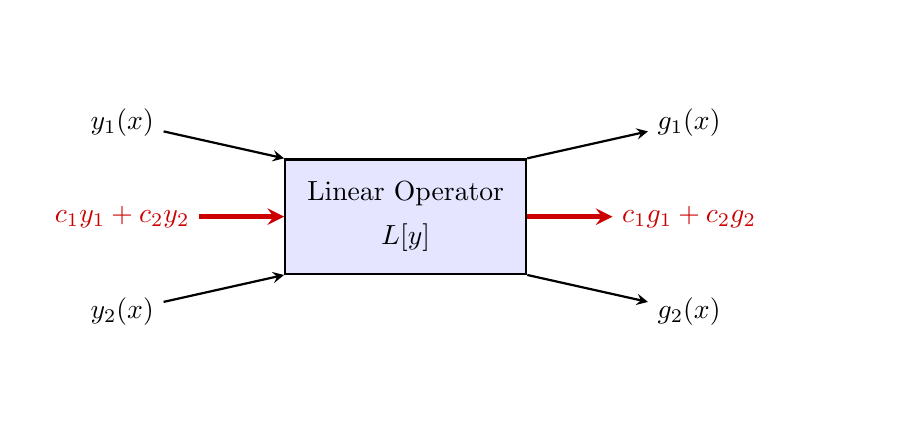
\begin{tikzpicture}[scale=1.2]
    \fill[white] (-1,-2) rectangle (8,2);
    \node[draw, thick, align=center, inner sep=8pt, fill=blue!10] (sys) at (3,0) {Linear Operator\\[4pt]$L[y]$};
    \node[align=center] (in1) at (0, 1) {$y_1(x)$};
    \node[align=center] (in2) at (0, -1) {$y_2(x)$};
    \node[align=center] (out1) at (6, 1) {$g_1(x)$};
    \node[align=center] (out2) at (6, -1) {$g_2(x)$};
    \draw[->, >=stealth, thick] (in1) -- (sys.north west);
    \draw[->, >=stealth, thick] (in2) -- (sys.south west);
    \draw[->, >=stealth, thick] (sys.north east) -- (out1);
    \draw[->, >=stealth, thick] (sys.south east) -- (out2);
    \node[align=center, red!80!black] (in3) at (0, 0) {$c_1 y_1 + c_2 y_2$};
    \node[align=center, red!80!black] (out3) at (6, 0) {$c_1 g_1 + c_2 g_2$};
    \draw[->, >=stealth, ultra thick, red!80!black] (in3) -- (sys.west);
    \draw[->, >=stealth, ultra thick, red!80!black] (sys.east) -- (out3);
\end{tikzpicture}
\end{center}

\textbf{Final Answers:}
\begin{itemize}
    \item $y_1' = \cos x$, $y_1'' = -\sin x$, $y_1''' = -\cos x$
    \item $y_2' = 2$, $y_2'' = 0$, $y_2''' = 0$
    \item (a) $y(x) = 5\sin x - 2x$
    \item (b) $y(x) = 10x - 5\sin x$
\end{itemize}

\newpage
\section{In-Depth Analysis of Problems and Techniques}

\subsection{Problem Types and General Approach}
The homework assignment can be categorized into four distinct problem types:
\begin{enumerate}
    \item \textbf{Existence and Uniqueness Intervals (Problems 1, 2):}
    \begin{itemize}
        \item \textit{Strategy:} Always divide by the leading coefficient $a_n(x)$ first to achieve standard form. Identify all points where any coefficient function $p_i(x)$ or the nonhomogeneous term $f(x)$ is undefined or discontinuous (e.g., division by zero, negative square roots). Plot these points on a number line to create open intervals. Select the single interval that contains the initial condition $x_0$.
    \end{itemize}
    \item \textbf{Linear Dependence vs. Independence (Problems 3, 4, 5):}
    \begin{itemize}
        \item \textit{Strategy:} Set up the equation $c_1 y_1 + c_2 y_2 + \dots + c_n y_n = 0$. If you can find non-zero constants that make the equation true for all $x$, they are dependent. If the only solution is $c_1 = c_2 = \dots = 0$, they are independent. For polynomials, group by powers of $x$. For trigonometric functions, evaluate at strategic points (like $\pi/2, \pi/4$) to create a system of equations for the constants.
    \end{itemize}
    \item \textbf{Wronskian and Fundamental Sets (Problem 6):}
    \begin{itemize}
        \item \textit{Strategy:} First, verify each function is a solution by plugging it into the ODE. Second, construct the $n \times n$ Wronskian matrix using the functions and their first $n-1$ derivatives. Calculate the determinant. If $W \neq 0$, they form a fundamental set.
    \end{itemize}
    \item \textbf{Initial Value Problems with Given Sets (Problems 7, 8):}
    \begin{itemize}
        \item \textit{Strategy:} Construct the general solution $y = y_c + y_p$. Differentiate this general solution $n-1$ times. Plug in the initial value $x_0$ to create a system of $n$ linear equations. Solve for $c_1, \dots, c_n$ and substitute back.
    \end{itemize}
    \item \textbf{Superposition Principle (Problem 9):}
    \begin{itemize}
        \item \textit{Strategy:} Recognize that if $L[y_1] = g_1$ and $L[y_2] = g_2$, then solving $L[y] = c_1 g_1 + c_2 g_2$ simply requires constructing the solution $y = c_1 y_1 + c_2 y_2$.
    \end{itemize}
\end{enumerate}

\subsection{Key Algebraic and Calculus Manipulations}
\begin{itemize}
    \item \textbf{Block Matrix Determinants (Problem 6):} Calculating a $4 \times 4$ determinant directly is tedious. By using row operations (adding Row 3 to Row 1, etc.), we created a block matrix with zeros in the top right quadrant. The determinant of a block lower triangular matrix $\begin{pmatrix} A & 0 \\ C & D \end{pmatrix}$ is simply $\det(A) \cdot \det(D)$. This trick saved massive amounts of computation time.
    \item \textbf{Polynomial Coefficient Matching (Problem 4):} To prove linear dependence of $\{x^2, x^2-1, 7\}$, we expanded the linear combination to $(c_1+c_2)x^2 + (-c_2+7c_3) = 0$. By setting the coefficients of each power of $x$ to zero, we transformed a functional equation into a simple linear algebra system.
    \item \textbf{Product Rule with Logarithms (Problem 8):} Differentiating $x(\ln x)^2$ requires careful application of the product and chain rules: $\frac{d}{dx}[x(\ln x)^2] = (1)(\ln x)^2 + x \cdot 2(\ln x) \cdot \frac{1}{x} = (\ln x)^2 + 2\ln x$. Missing the chain rule on $(\ln x)^2$ is a common trap.
\end{itemize}

\newpage
\section{"Cheatsheet" and Tips for Success}

\renewcommand{\arraystretch}{1.5}
\begin{table}[h]
\centering
\begin{tabularx}{\textwidth}{>{\hsize=0.3\hsize}X >{\hsize=0.7\hsize}X}
\toprule
\textbf{Concept} & \textbf{Formula / Rule} \\
\midrule
\textbf{Standard Form} & $y^{(n)} + p_{n-1}(x)y^{(n-1)} + \dots + p_0(x)y = f(x)$ \\
\addlinespace[4pt]
\textbf{Wronskian} & $W = \det \begin{pmatrix} y_1 & \dots & y_n \\ \vdots & \ddots & \vdots \\ y_1^{(n-1)} & \dots & y_n^{(n-1)} \end{pmatrix}$ \\
\addlinespace[4pt]
\textbf{Superposition} & If $L[y_1] = g_1$ and $L[y_2] = g_2$, then $L[c_1 y_1 + c_2 y_2] = c_1 g_1 + c_2 g_2$ \\
\addlinespace[4pt]
\textbf{General Solution} & $y(x) = c_1 y_1(x) + \dots + c_n y_n(x) + y_p(x)$ \\
\bottomrule
\end{tabularx}
\end{table}

\subsection{Cheats and Shortcuts}
\begin{itemize}
    \item \textbf{The Exponential Shortcut:} Any set of exponential functions $e^{r_1 x}, e^{r_2 x}, \dots$ with strictly distinct constants $r_i$ is \textit{always} linearly independent. You do not need to calculate the Wronskian to know this; it is a mathematical guarantee.
    \item \textbf{The Zero-Root Trick:} When evaluating initial value problems at $x=1$ involving $\ln x$ (like in Problem 8), remember that $\ln(1) = 0$. This immediately annihilates many terms in your system of equations, making it much easier to solve. Always scan for terms that will zero out before doing heavy algebra.
\end{itemize}

\subsection{Common Pitfalls and Traps}
\begin{itemize}
    \item \textbf{The Leading Coefficient Trap:} In Existence/Uniqueness problems, the most common mistake is forgetting to divide by $a_n(x)$. If you look at $x y'' + y = 0$, you might think the interval is $(-\infty, \infty)$ because $x$ and $1$ are continuous everywhere. But standard form is $y'' + \frac{1}{x}y = 0$, revealing a massive discontinuity at $x=0$.
    \item \textbf{Wronskian Misinterpretation:} If $W = 0$, the functions are linearly dependent \textit{only if} they are known to be solutions to a linear homogeneous ODE. If you are just given random functions, $W=0$ does not strictly guarantee dependence.
    \item \textbf{Non-Linear Superposition:} Superposition \textit{only} works for linear equations. You cannot use it for equations like $y'' + y^2 = 0$.
\end{itemize}

\newpage
\section{Conceptual Synthesis and The "Big Picture"}

\subsection{Thematic Connections}
The central theme of this chapter is \textbf{Linearity and Vector Spaces}. While calculus deals with rates of change, this specific topic is actually a disguised linear algebra course. The set of all solutions to an $n$-th order homogeneous linear ODE forms an $n$-dimensional vector space. 
Just as any vector in 3D space can be written as a linear combination of basis vectors $\hat{i}, \hat{j}, \hat{k}$, any solution to a 3rd-order ODE can be written as a linear combination of a "basis" of functions (the fundamental solution set). The Wronskian is simply the functional equivalent of checking if vectors are coplanar.

\subsection{Forward and Backward Links}
\begin{itemize}
    \item \textbf{Backward Links:} This topic builds directly on First-Order Linear Equations (integrating factors). The concept of a general solution being $y_c + y_p$ was introduced there, but is now expanded to $n$ dimensions.
    \item \textbf{Forward Links:} Understanding fundamental sets is the absolute prerequisite for the next major topics: \textbf{Undetermined Coefficients} and \textbf{Variation of Parameters}. In Variation of Parameters, you will actually use the Wronskian determinant in the denominator of an integral to construct the particular solution $y_p$. If you cannot compute a Wronskian now, you will not be able to integrate later.
\end{itemize}

\section{Abstract Real-World Modeling (AI, ML, \& Quant Finance)}

\subsection{Concrete Scenarios}
Higher-order linear differential equations are not just theoretical; they govern complex dynamics in advanced computational fields:
\begin{enumerate}
    \item \textbf{Machine Learning (Optimization Dynamics):} Gradient descent can be modeled as a 1st-order ODE. Adding "momentum" (Heavy Ball method) turns it into a 2nd-order ODE. Adding "jerk" (Nesterov acceleration or higher-order smoothing) models the optimization trajectory as a 3rd-order linear ODE, allowing researchers to prove convergence rates.
    \item \textbf{Quantitative Finance (Stochastic Interest Rates):} While Black-Scholes is a 2nd-order PDE, advanced models for interest rate term structures (like the Hull-White model) often involve higher-order linear stochastic differential equations (SDEs) to capture mean-reversion and volatility clustering over time.
\end{enumerate}

\subsection{Model Problem Setup: 3rd-Order Optimization Dynamics in ML}
Let us model the continuous-time limit of a machine learning optimization algorithm with momentum and jerk. Let $\theta(t)$ be the parameter weight of a neural network at time $t$. We are minimizing a quadratic loss function $L(\theta) = \frac{1}{2} k \theta^2$, meaning the gradient is $\nabla L = k\theta$.

A standard gradient descent with momentum follows $\theta'' + \gamma \theta' + k\theta = 0$. To prevent aggressive oscillations (over-shooting the minimum), we introduce a jerk penalty $\alpha \theta'''$, leading to a 3rd-order linear homogeneous ODE:
\[ \theta''' + \alpha \theta'' + \beta \theta' + k \theta = 0 \]
where $\alpha, \beta, k > 0$ are hyperparameters. 

To ensure the neural network converges to the global minimum $\theta = 0$ without diverging, the roots of the characteristic equation $r^3 + \alpha r^2 + \beta r + k = 0$ must all have strictly negative real parts. By analyzing the fundamental solution set $\{e^{r_1 t}, e^{r_2 t}, e^{r_3 t}\}$, AI researchers can tune $\alpha$ and $\beta$ to achieve critical damping, ensuring the fastest possible training time without instability.

\newpage
\section{Common Variations and Untested Concepts}

Based on standard curriculum, here are important concepts related to Section 6.1 that were not explicitly tested in your homework:

\subsection{Abel's Identity}
Abel's Identity provides a way to find the Wronskian of a fundamental set of solutions \textit{without} knowing the solutions themselves, using only the coefficients of the ODE.
\textbf{Theorem:} For $y^{(n)} + p_{n-1}(x)y^{(n-1)} + \dots + p_0(x)y = 0$, the Wronskian is given by:
\[ W(x) = C \exp\left( -\int p_{n-1}(x) \, dx \right) \]
where $C$ is a constant.

\textbf{Example:} Find the Wronskian of the fundamental set for $y'' - \frac{2}{x}y' + e^x y = 0$ (up to a constant).
\textit{Solution:} Here, $p_1(x) = -\frac{2}{x}$. Using Abel's Identity:
\[ W(x) = C \exp\left( -\int -\frac{2}{x} \, dx \right) = C \exp(2 \ln x) = C x^2 \]

\subsection{Reduction of Order for Higher-Order ODEs}
If you know one solution $y_1(x)$ to a linear homogeneous ODE, you can find a second linearly independent solution by substituting $y_2(x) = u(x)y_1(x)$ into the ODE, which reduces the order of the equation for $u'$.

\section{Advanced Diagnostic Testing: "Find the Flaw"}

Below are 5 problems with subtle, critical flaws in their solutions. Your task as a student is to find the error, explain it, and correct it.

\textbf{Problem 1:} Find the largest interval for a unique solution to $x y'' + y = 0, \quad y(-2)=1, \quad y'(-2)=0$.
\textit{Flawed Solution:} The coefficient functions are $p_1(x)=x$ and $p_0(x)=1$. Both are polynomials and continuous everywhere. Therefore, the interval is $(-\infty, \infty)$.
\textit{Correction:} The flaw is failing to put the equation in standard form. Dividing by $x$ gives $y'' + \frac{1}{x}y = 0$. The discontinuity is at $x=0$. The interval containing $x_0 = -2$ is $(-\infty, 0)$.

\textbf{Problem 2:} Determine if $f_1(x) = x^2$ and $f_2(x) = x|x|$ are linearly dependent on $[-1, 1]$.
\textit{Flawed Solution:} The Wronskian is $W = (x^2)(2|x|) - (x|x|)(2x) = 2x^2|x| - 2x^2|x| = 0$. Since $W=0$, they are linearly dependent.
\textit{Correction:} $W=0$ only guarantees dependence if the functions are solutions to a linear ODE. These are not. They are actually independent on $[-1, 1]$ because $c_1 x^2 + c_2 x|x| = 0$ requires $c_1=c_2=0$ (check $x=1$ and $x=-1$).

\textbf{Problem 3:} Use superposition to find a solution to $y'' + y^2 = 0$.
\textit{Flawed Solution:} Let $y_1$ and $y_2$ be solutions. By the superposition principle, $y = c_1 y_1 + c_2 y_2$ is also a solution.
\textit{Correction:} Superposition only applies to \textit{linear} differential equations. The $y^2$ term makes this equation non-linear, so superposition fails.

\textbf{Problem 4:} Are $\{1, \sin^2 x, \cos^2 x\}$ linearly independent?
\textit{Flawed Solution:} Set $c_1(1) + c_2 \sin^2 x + c_3 \cos^2 x = 0$. At $x=0$, $c_1+c_3=0$. At $x=\pi/2$, $c_1+c_2=0$. Solving this yields $c_1=c_2=c_3=0$. They are independent.
\textit{Correction:} The student made an algebra error. Since $\sin^2 x + \cos^2 x = 1$, we have $1(1) - 1(\sin^2 x) - 1(\cos^2 x) = 0$. They are linearly dependent.

\textbf{Problem 5:} Find the general solution to $y''' - y'' = 0$.
\textit{Flawed Solution:} Characteristic equation $r^3 - r^2 = 0 \implies r^2(r-1) = 0$. Roots are $0, 0, 1$. Solution is $y = c_1 e^{0x} + c_2 e^{0x} + c_3 e^x = (c_1+c_2) + c_3 e^x = C + c_3 e^x$.
\textit{Correction:} Repeated roots require multiplying by $x$ to maintain linear independence. The correct solution is $y = c_1 + c_2 x + c_3 e^x$.

\end{document}